% Some LaTeX commands I define for my own nomenclature.
% If you have to, it's better to change nomenclature once here than in a 
% million places throughout your thesis!
\newcommand{\package}[1]{\textbf{#1}} % package names in bold text
\newcommand{\cmmd}[1]{\textbackslash\texttt{#1}} % command name in tt font 


%======================================================================
\chapter{Model Description}
%======================================================================

The model is composed of human population given by $N_{h}$ and
reservoir population given by $N_{r}$. We divide the human population ($N_{h}$) in $5$ categories namely, Susceptibles ($S_{h}$), Vaccinated ($V_{h}$), Exposed ($E_{h}$), Infected ($I_{h}$) and Recovered ($R_{h}$) whereas the reservoir population ($N_{r}$) is divided among Susceptibles ($S_{r}$), Infected($I_{r}$) and Recovered ($R_{r}$), such that
\[N_{h} = S_{h} + V_{h} + E_{h} + I_{h} + R_{h}\]
\[N_{r} = S_{r} + I_{r} + R_{r}\]

\begin{figure}[h]
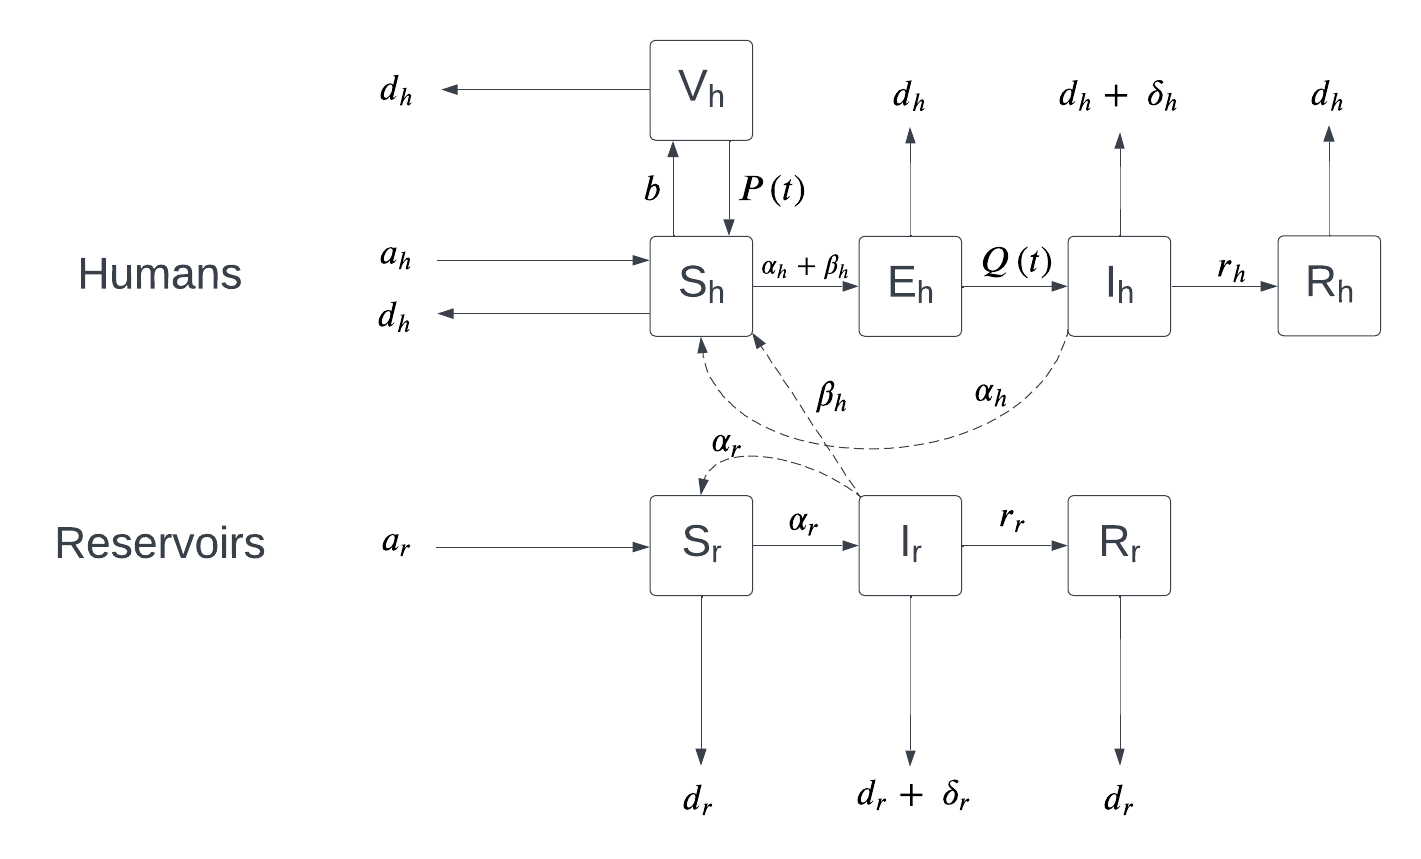
\includegraphics[width=\textwidth]{flow-diagram}
\caption{Model Flow Diagram}
\centering
\end{figure}
We assume that $a_{h}$ and $a_{r}$ is the constant birth rate of susceptible humans and reservoirs respectively and susceptibles are vaccinated at a constant rate $b$. $\alpha_{r}$, $\alpha_{h}$ and $\beta_{h}$ are the infection rates from reservoir to reservoir, reservoir to human and from human to human respectively.
To allow for a general latent period, we further assume that $P(t)$ is the probability of individuals remaining in the vaccinated class $t$ units after being vaccinated and $Q(t)$ is the probability of individuals remaining in the exposed class $t$ units after being exposed to the monkeypox virus. $r_{h}$ and $r_{r}$ are the recovery rates of the humans and the reservoirs respectively from the infection. Lastly, we consider that $d_{h}$ and $\delta_{h}$ is the natural and infection related death rate of humans whereas $d_{r}$ and $\delta_{r}$ is the natural and infection-related death rate of reservoirs.
According to the natural progression of the disease, we assume $P(t)$ and $Q(t)$ non-negative, non-increasing and piecewise continuous with 
\begin{center}
$P(0^{+}) = Q(0^{+}) = 1$ and $P(\infty) = Q(\infty) = 0$
\end{center}



